\section{Preprocessing}
\label{sec:preprocessing}

Come discusso nel Capitolo~\ref{ch:introduzione}, la fase di preprocessing ha l'obiettivo di rendere il modello CAD quanto più consistente possibile prima dell'elaborazione. Si interviene correggendo i layer, blocchi, geometrie e ridondanze.

Come caso di studio prendiamo il modello DXF selezionato e lo apriamo con LibreCAD per analizzarlo.

\begin{figure}[htbp]
	\centering
	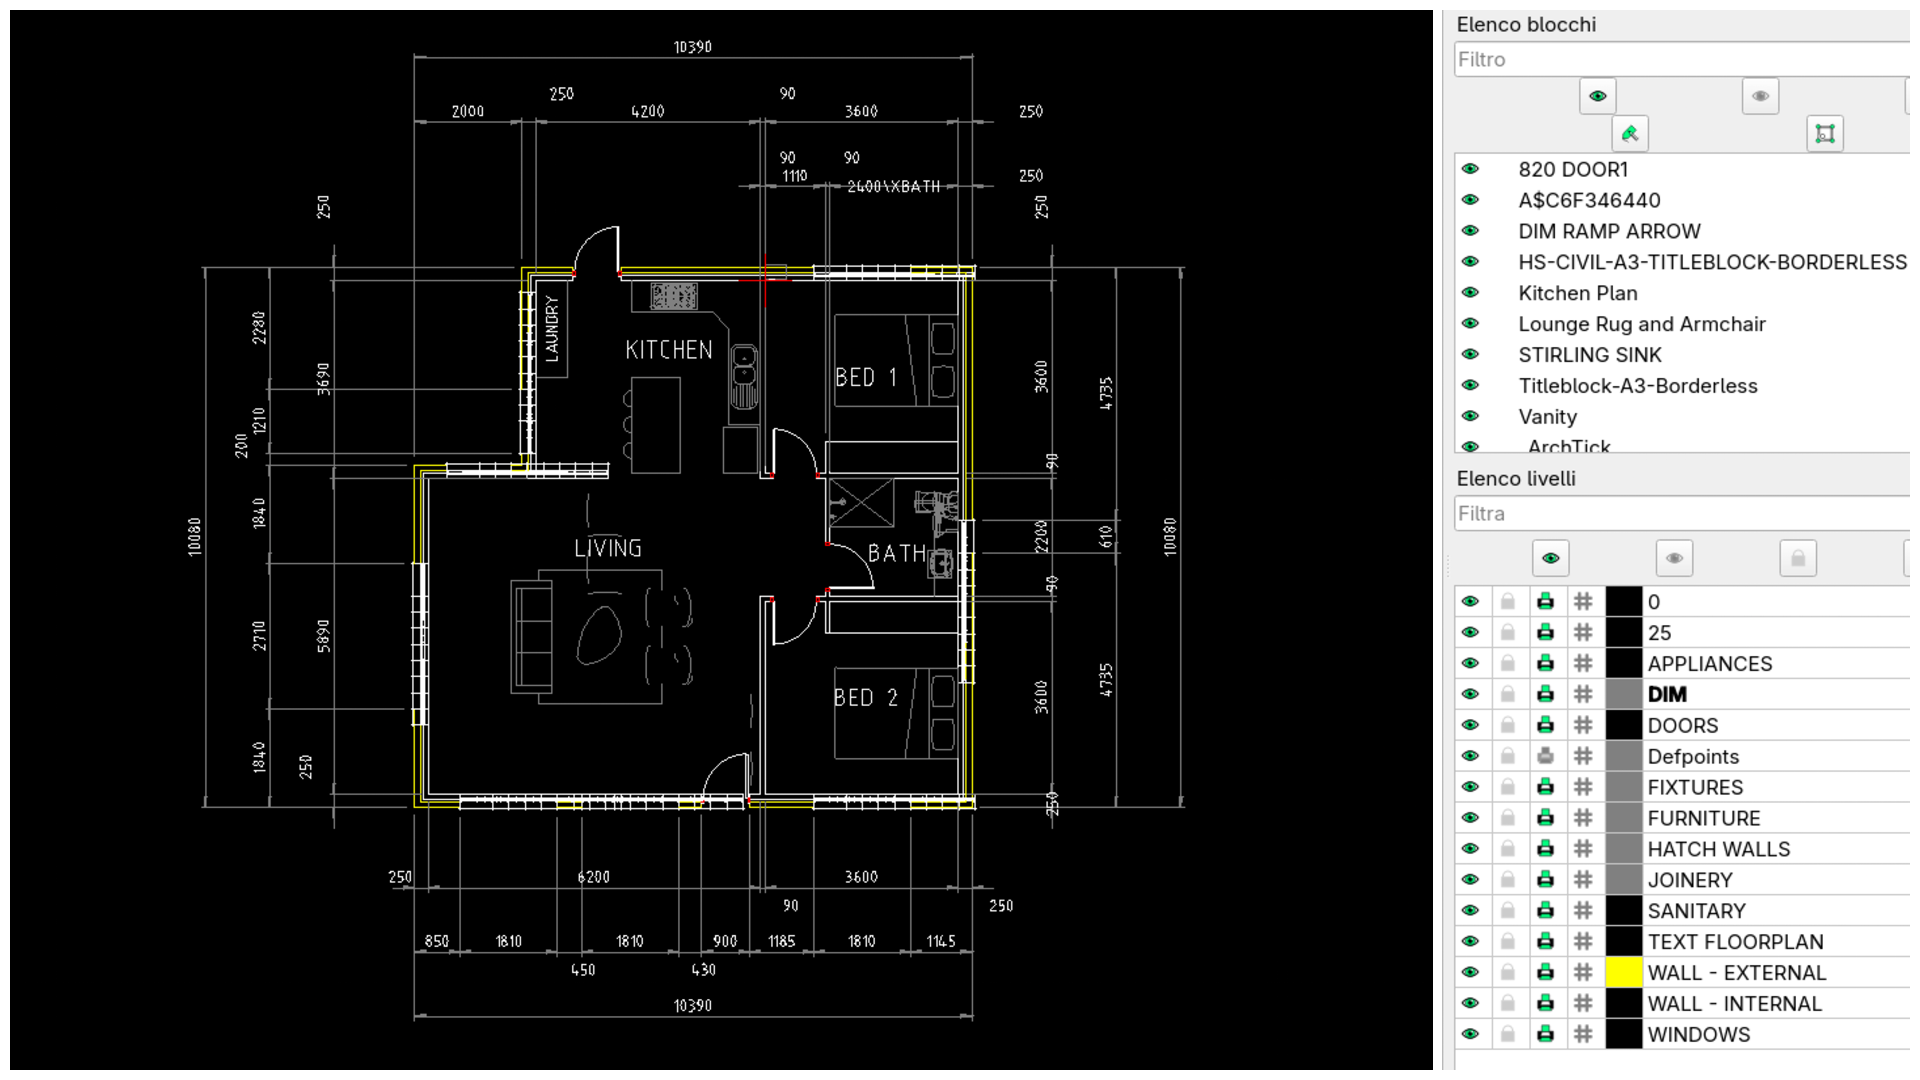
\includegraphics[width=1\textwidth]{images/02_geometry_processing/screen001.png}
	\caption{Modello CAD di caso di studio aperto in LibreCAD.}
	\label{fig:screen001}
\end{figure}

Isoliamo inizialmente solo i layer relativi ai muri e osserviamo che sono presenti due layer distinti: \texttt{WALL EXTERNAL} (evidenziato in giallo) e \texttt{WALL INTERNAL}. I segmenti del layer \texttt{WALL EXTERNAL} risultano ridondanti e possono essere rimossi senza alcun impatto sulla geometria finale. Osserviamo inoltre che le primitive dei muri non sono polilinee chiuse, bensì segmenti che formano contorni aperti: la geometria risulta quindi incompleta e necessita di correzione. Sono infine presenti due ulteriori segmenti isolati, che costituiscono rumore e possono anch'essi essere rimossi.

\begin{figure}[htbp]
	\centering
	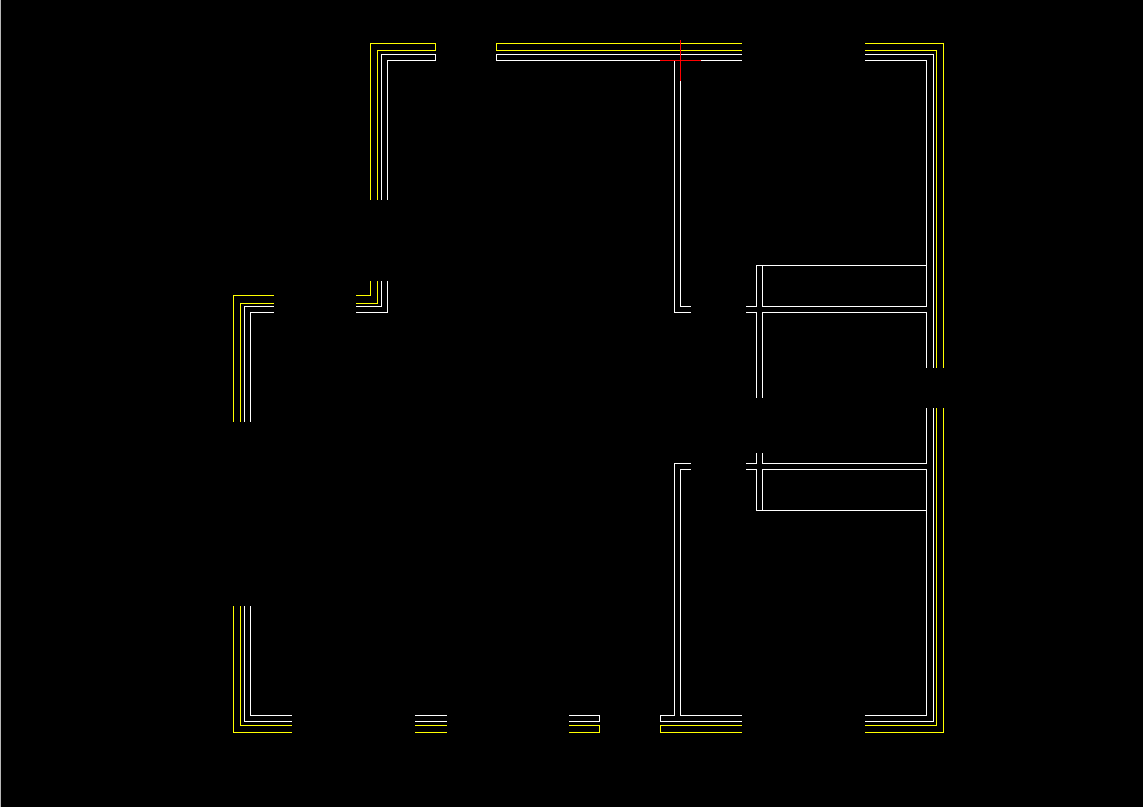
\includegraphics[width=0.7\textwidth]{images/02_geometry_processing/screen002.png}
	\caption{Layer dei muri prima della correzione: si notano il layer ridondante \texttt{WALL EXTERNAL}, i contorni aperti e i segmenti isolati.}
	\label{fig:screen002}
\end{figure}

Dopo aver corretto questi problemi, otteniamo la rappresentazione dei muri mostrata in figura:

\begin{figure}[htbp]
	\centering
	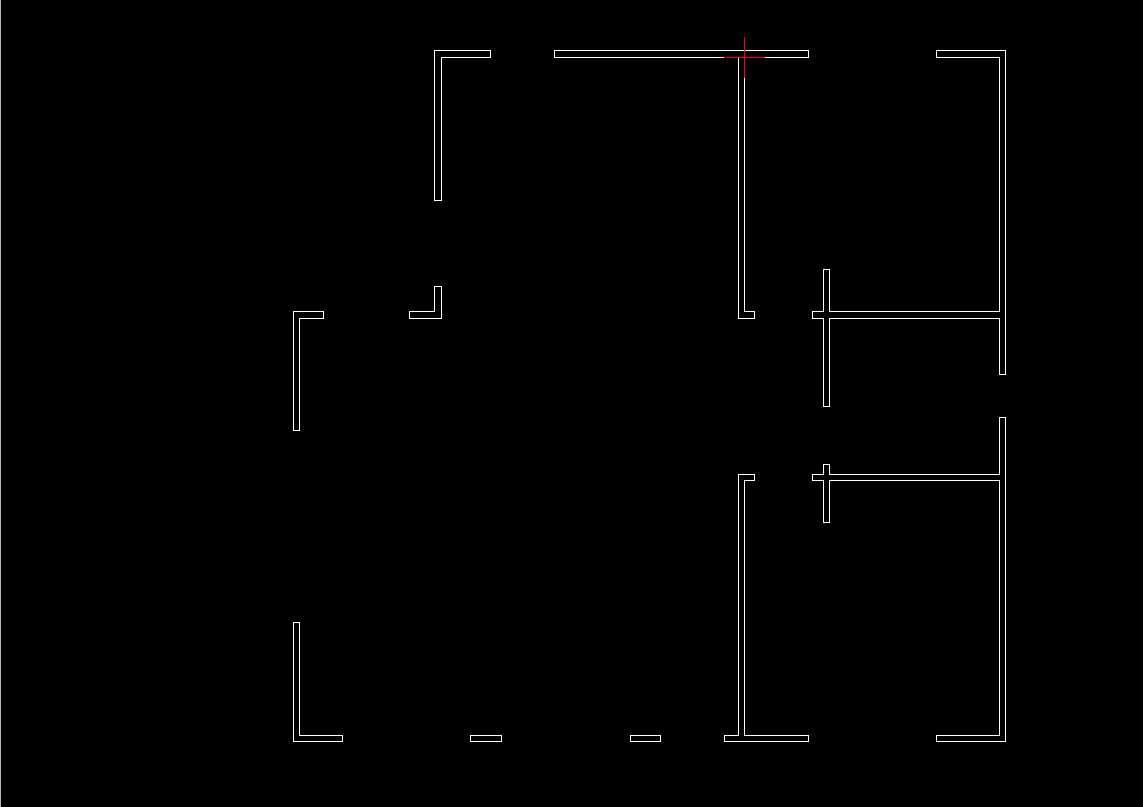
\includegraphics[width=0.7\textwidth]{images/02_geometry_processing/screen003.png}
	\caption{Layer dei muri dopo la correzione.}
	\label{fig:screen003}
\end{figure}

Nonostante i muri siano ancora separati tra loro, a causa della presenza di porte e finestre, quello che otteniamo è un insieme di poligoni chiusi. Analizziamo a questo punto le finestre: osserviamo come non siano rappresentate in una forma adeguata. Ogni finestra è descritta come un blocco (\texttt{BLOCK}) contenente centinaia di segmenti; inoltre, due finestre risultano sovrapposte tra loro, e due di queste fuoriescono addirittura dalle mura.

\begin{figure}[htbp]
	\centering
	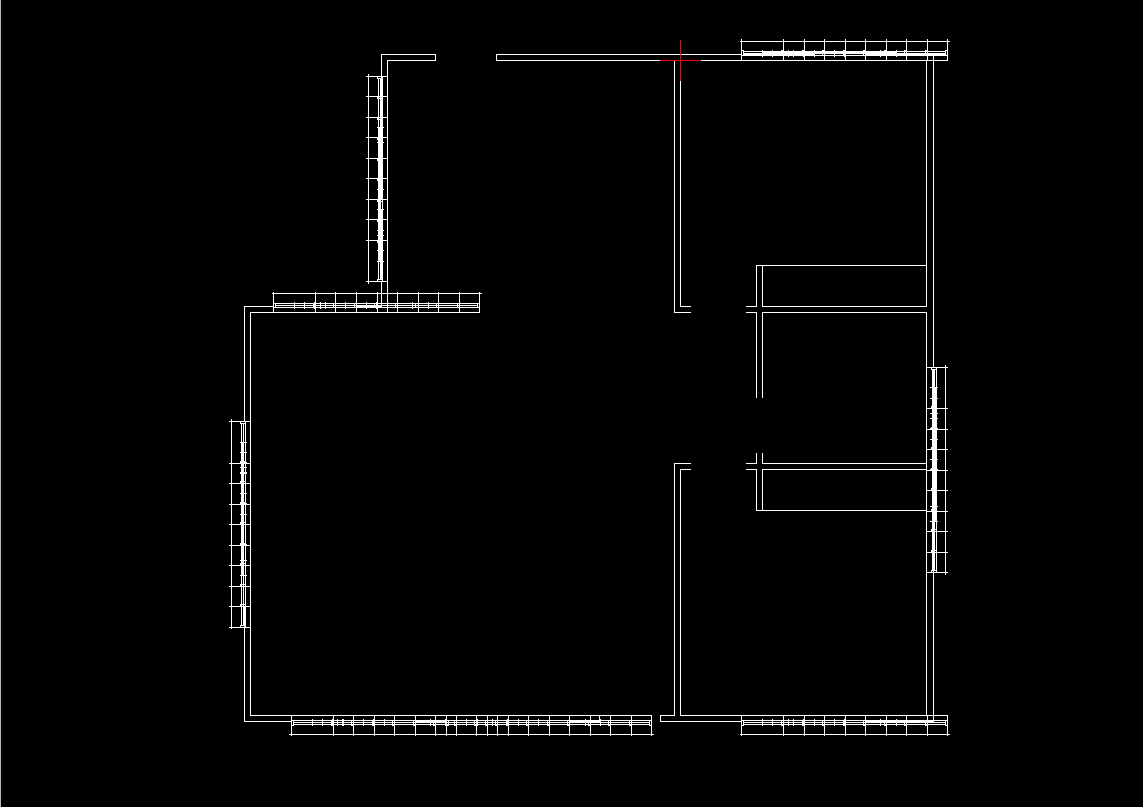
\includegraphics[width=0.7\textwidth]{images/02_geometry_processing/screen004.png}
	\caption{Rappresentazione originale delle finestre: si notano il blocco composto da centinaia di segmenti, la sovrapposizione tra due finestre e una finestra che invade lo spazio interno.}
	\label{fig:screen004}
\end{figure}

Dopodiché, i layer sono stati rinominati in modo coerente: \texttt{A-WALL} per i muri, \texttt{A-DOOR} per le porte e \texttt{A-WINDOW} per le finestre. Tutti gli altri layer, non essendo rilevanti per la ricostruzione della geometria, sono stati esclusi. Anche i blocchi sono stati rinominati: un blocco per la porta (\texttt{BLOCK-DOOR-1}) e quattro blocchi per le finestre (\texttt{BLOCK-WINDOW-1}, \ldots, \texttt{BLOCK-WINDOW-4}).

\begin{figure}[htbp]
	\centering
	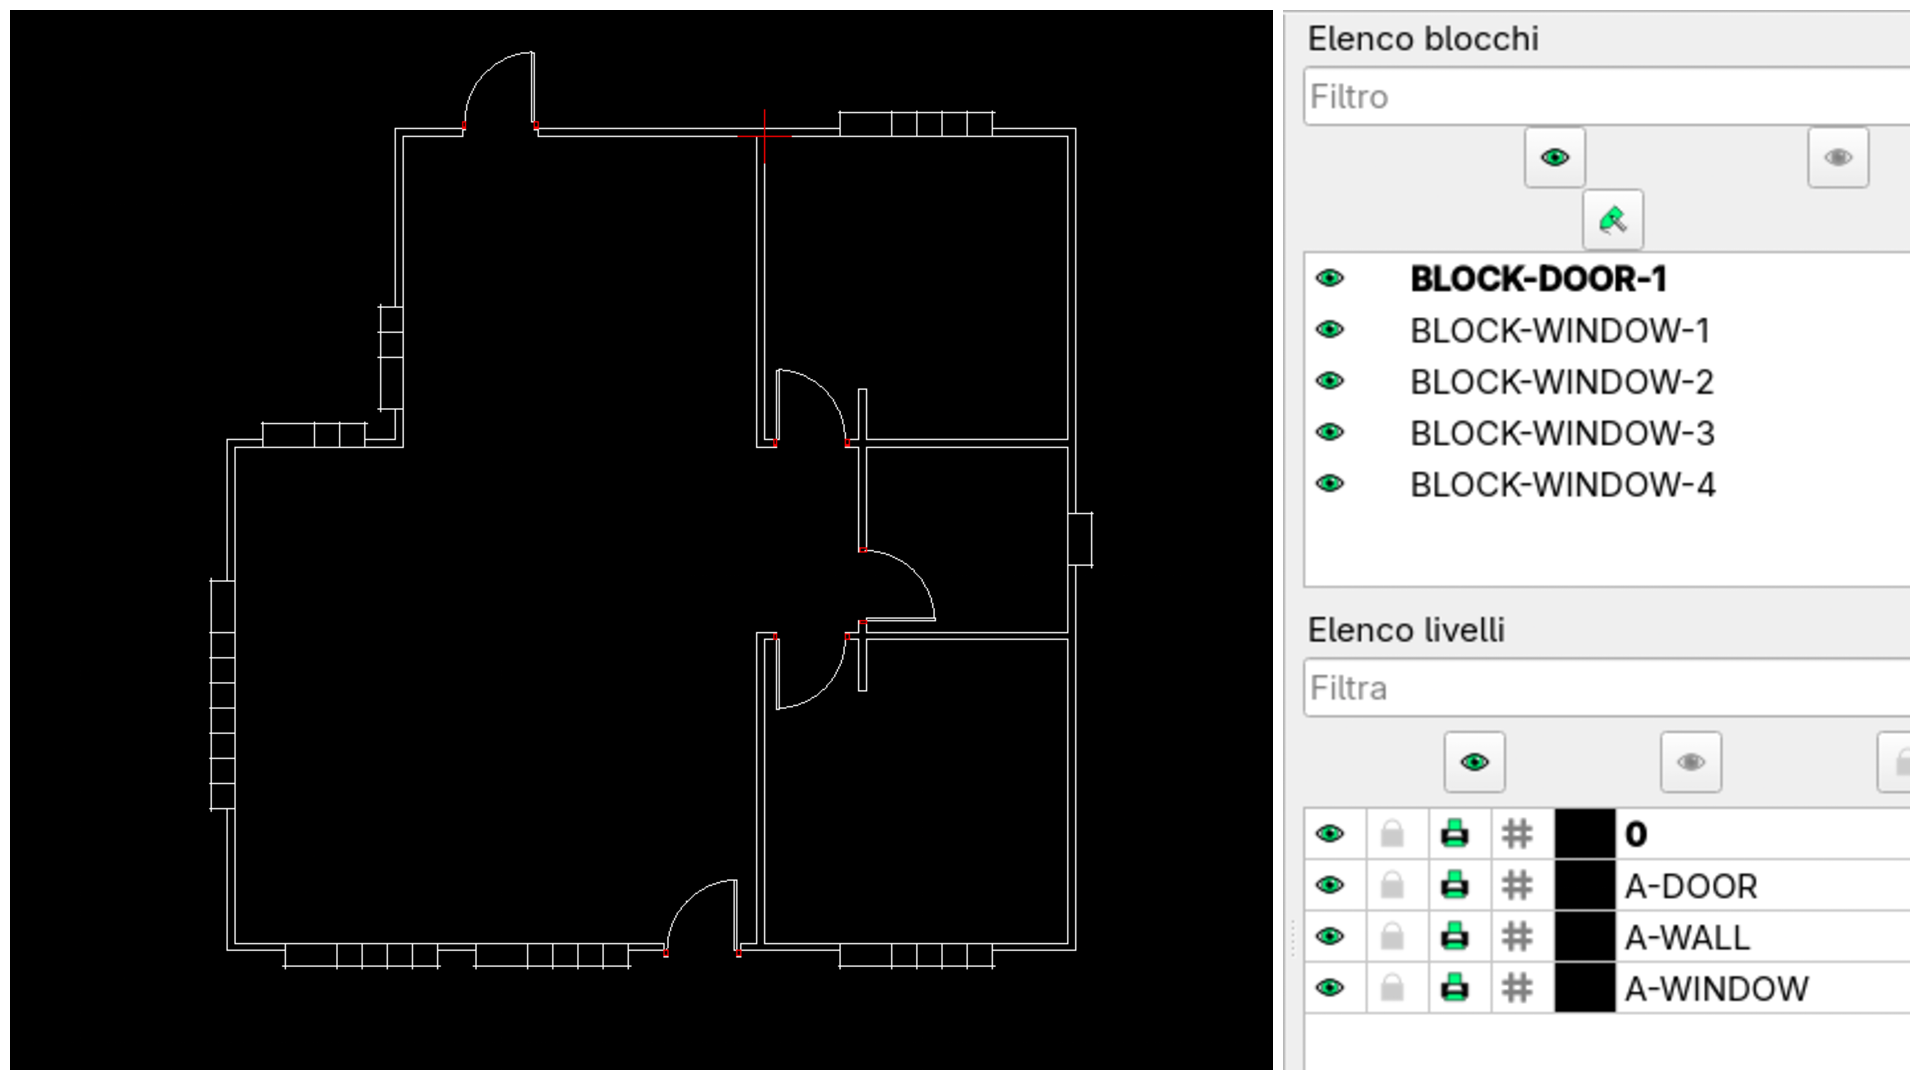
\includegraphics[width=0.7\textwidth]{images/02_geometry_processing/screen005.png}
	\caption{Rappresentazione delle finestre dopo la correzione.}
	\label{fig:screen005}
\end{figure}
